\caulc
%%%=============EX_1=============%%%
\begin{ex}%[1D2N2-4]%[TDMZZ14-1-TN]%[Mui Doan]
	Cho cấp số cộng $(u_n)$ có số hạng thứ nhất bằng $3$ và công sai bằng $-1$. Số hạng thứ ba của $(u_n)$ bằng
	\choice
	{$2$}
	{$0$}
	{$5$}
	{\True $1$}
	\loigiai{
		Ta có $u_3=u_1+2d=3+2\cdot (-1)=1$.
	}
\end{ex}
%%%=============================%%%

%%%=============EX_2=============%%%
\begin{ex}%[1D7N2-1]%[TDMZZ14]%[Nguyễn Sơn Thành]
	Đạo hàm của hàm số $y = \ln x$ với $x > 0$ là
	\choice
	{$y' = -\dfrac{1}{x}$}
	{$y' = \dfrac{1}{x \ln 2}$}
	{\True $y' = \dfrac{1}{x}$}
	{$y' = \dfrac{1}{x^2}$}
	\loigiai{
		Áp dụng công thức đạo hàm cơ bản của hàm số lô-ga-rít tự nhiên
		\[(\ln x)' = \dfrac{1}{x}, \forall x > 0.\]
		Vậy đạo hàm của hàm số đã cho là $y' = \dfrac{1}{x}$.
	}
\end{ex}
%%%=============================%%%

%%%=============EX_3=============%%%
\begin{ex}%[1D6H4-5]%[TDMZZ14]%[Phạm Hải Dương]
	Tập nghiệm của bất phương trình $3^{x^2-2x} \le 27$ là
	\choice
	{$[-3;1]$}
	{$\varnothing$}
	{$[1;3]$}
	{\True $[-1;3]$}
	\loigiai{
		Ta có
		\begin{eqnarray*}
			&& 3^{x^2-2x} \le 27\\ 
			&\Leftrightarrow& 3^{x^2-2x} \le 3^3\\
			&\Leftrightarrow& x^2 - 2x \le 3\\
			&\Leftrightarrow& x^2 - 2x - 3 \le 0\\
			&\Leftrightarrow& -1 \le x \le 3.
		\end{eqnarray*}
		Vậy tập nghiệm của bất phương trình là $S=[-1;3]$.
	}
\end{ex}
%%%=============================%%%

%%%=============EX_4=============%%%
\begin{ex}%[1H8N7-5]%[GVBS: Trần Phi Thoàn]
	Cho hình lăng trụ đều $ABCD.A'B'C'D'$ có đáy là hình vuông cạnh bằng $2$ và cạnh bên $AA'=3\pi$. Thể tích của khối lăng trụ $ABC.A'B'C'$ bằng
	\choice
	{$12$}
	{$12\pi$}
	{$6$}
	{\True $6\pi$}
	\loigiai{
		Thể tích khối lăng trụ đều $ABCD.A'B'C'D'$ là
		\[V_{ABCD.A'B'C'D'}=AA'\cdot S_{ABCD}=3\pi\cdot 2^2=12\pi.\]
		Mà $V_{ABC.A'B'C'}=\dfrac{1}{2}V_{ABCD.A'B'C'D'}$.\\
		Vậy $V_{ABC.A'B'C'}=6\pi$.
	}
\end{ex}
%%%=============================%%%

%%%=============EX_5=============%%%
\begin{ex}%[2D1N1-2]%[TDMZZ14]%[Nguyễn Tấn Linh]
	\immini[thm]{Cho đồ thị hàm số $y=f(x)$ như hình vẽ bên dưới. Hỏi hàm số $f(x)$ nghịch biến trên khoảng nào dưới đây?
		\choice
		{\True $(0;4)$}
		{$(4;5)$}
		{$(-\infty;0)$}
		{$(4;+\infty)$}
	}
	{
		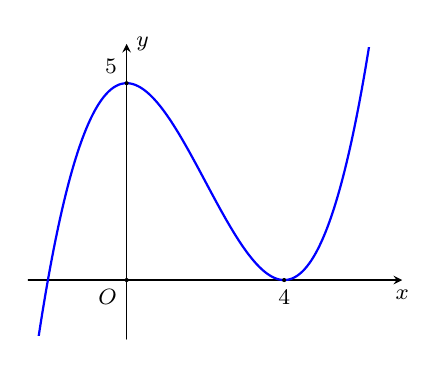
\begin{tikzpicture}[line join=round, line cap=round, >=stealth, font=\footnotesize, scale=0.5, declare function={f(\x)=5/32*(\x)^3-15/16*(\x)^2+5;}]
			\def\xt{-2.5} \def\xp{7} \def\yd{-1.5} \def\yt{6}
			\draw[->] (\xt,0)--(\xp,0) node[below,black]{$x$};
			\draw[->] (0,\yd)--(0,\yt) node[right,black]{$y$};
			\fill (0,0) circle (1.5pt) node[below left]{$O$};
			\begin{scope}
				\clip (\xt+0.1,\yd+0.1) rectangle (\xp-0.1,\yt-0.1);
				\draw[samples=150,smooth,domain=\xt:\xp,blue,thick] plot(\x,{f(\x)});
			\end{scope}
			\fill (0,5) circle (1.5pt) node[black,above left]{$5$};
			\fill (4,0) circle (1.5pt) node[black,below]{$4$};
		\end{tikzpicture}
	}
	\loigiai{
		Dựa vào đồ thị, ta thấy hàm số $f(x)$ nghịch biến trên khoảng $(0;4)$.
	}
\end{ex}
%%%=============================%%%

%%%=============EX_6=============%%%
\begin{ex}%[2D4N2-1]%[TDMZZ14]%[Bồ Văn Hậu]
	Biết $\displaystyle\int\limits_0^1 f(x)\mathrm{\,d}x = 2$ và $\displaystyle\int\limits_1^3 f(x)\mathrm{\,d}x = 4$. Giá trị $\displaystyle\int\limits_0^3 f(x)\mathrm{\,d}x$ bằng
	\choice
	{$8$}
	{\True $6$}
	{$-2$}
	{$0$}
	\loigiai{
		Ta có $\displaystyle\int\limits_0^3 f(x)\mathrm{\,d}x= \displaystyle\int\limits_0^1 f(x)\mathrm{\,d}x+ \displaystyle\int\limits_1^3 f(x)\mathrm{\,d}x=2+4=6$.
	}
\end{ex}
%%%=============================%%%

%%%=============EX_7=============%%%
\begin{ex}%[2D4N3-1]%[TDMZZ14]%[Bồ Văn Hậu]
	Cho hình phẳng $(H)$ giới hạn bởi các đường $y=f(x)$, $Ox$, $x=a$, $x=a-1$ với $a$ là số thực. Diện tích hình phẳng $(H)$ được tính theo công thức
	\choice
	{$S=\displaystyle\int\limits_a^{a-1}\left|f(x)\right|\mathrm{\,d}x$}
	{$S=\displaystyle\int\limits_{a-1}^a f(x)\mathrm{\,d}x$}
	{$S=-\displaystyle\int\limits_a^{a-1} f(x)\mathrm{\,d}x$}
	{\True $S=\displaystyle\int\limits_{a-1}^a\left|f(x)\right|\mathrm{\,d}x$}
	\loigiai{
		Hình phẳng $(H)$ giới hạn bởi các đường $y=f(x)$, $Ox$, $x=a$, $x=a-1$ có diện tích là
		\[S = \displaystyle\int\limits_{a-1}^a |f(x)|\mathrm{\,d}x.\]
	}
\end{ex}
%%%=============================%%%

%%%=============EX_8=============%%%
\begin{ex}%[2D1H5-5]%[TDMZZ14]%[Lê Phúc]
	\immini[thm]{Cho hàm số $y=f(x)$ có đồ thị hàm số $y=f'(x)$ như hình vẽ bên dưới. Hỏi hàm số $f(x)$ có thể làm hàm số nào dưới đây?
		\choice
		{$f(x)=ax^4+bx^2+c$}
		{\True $f(x)=ax^4+bx^3+cx^2+dx+m$}
		{$f(x)=ax^3+bx^2+cx+d$}
		{$f(x)=\dfrac{ax+b}{cx+d}$}
	}
	{	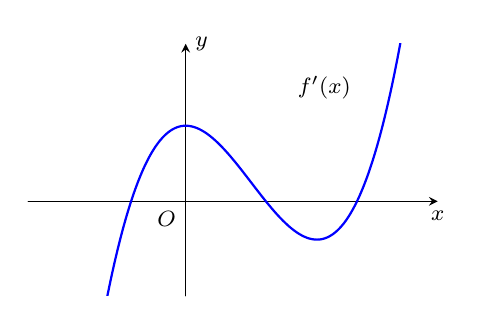
\begin{tikzpicture}[>=stealth,scale=0.8, font=\footnotesize, line join=round,line cap=round]
			% --- Hệ trục tọa độ ---
			\draw[->] (-2.5,0)--(4,0) node[below]{$x$};
			\draw[->] (0,-1.5)--(0,2.5) node[right]{$y$};
			\node[below left] at (0,0) {$O$};
			% --- Vẽ đồ thị f'(x) ---
			\begin{scope}
				\clip (-2.5,-1.5) rectangle (4,2.5);
				\draw[line width=0.8,blue, smooth, samples=150, domain=-2.2:4]
				plot (\x,{0.4*(\x)^3 - 1.25*(\x)^2 + 1.2});
				\node at (2.2,1.8) {$f'(x)$};
			\end{scope}
	\end{tikzpicture}}
	\loigiai{
		Dựa vào đồ thị hàm số $y=f'(x)$, ta thấy đồ thị có hai cực trị và không đối xứng qua $O$.\\
		Suy ra hàm số $f'(x)$ là hàm số bậc ba.\\
		Mà $f(x)$ là một nguyên hàm của $f'(x)$ nên $f(x)$ là hàm số bậc bốn.\\
		Xét $f(x)=ax^4+bx^2+c$.\\
		Ta có $f'(x)=4ax^3+2bx$ là hàm số lẻ nên đồ thị của hàm số $y=f'(x)$ nhận gốc tọa độ $O$ làm tâm đối xứng, suy ra đồ thị $f'(x)$ không thể có dạng như hình vẽ (không thỏa mãn).\\
		Vậy hàm số $f(x)$ có thể là $f(x)=ax^4+bx^3+cx^2+dx+m$.
	}
\end{ex}
%%%=============================%%%

%%%=============EX_9=============%%%
\begin{ex}%[2H2N2-1]%[TDMZZ14]%[GVBS: Corrected]
	Trong không gian $Oxyz$, độ dài của vectơ $\overrightarrow{u}=(2;4;4)$ bằng
	\choice
	{$10$}
	{$4\sqrt{5}$}
	{$3$}
	{\True $6$}
	\loigiai{
		Ta có $|\overrightarrow{u}| = \sqrt{2^2 + 4^2 + 4^2} = \sqrt{4 + 16 + 16} = \sqrt{36} = 6$.
	}
\end{ex}
%%%=============================%%%

%%%=============EX_10=============%%%
\begin{ex}%[2H5H1-2]%[TDMZZ14]%[Võ Hiệp]
	Trong không gian $Oxyz$, cho mặt phẳng $(\alpha)\colon \dfrac{x}{2} + \dfrac{y}{3} - \dfrac{z}{6} = 1$. Một vectơ pháp tuyến của mặt phẳng $(\alpha)$ có tọa độ là
	\choice
	{$(3;2;1)$}
	{$(2;3;-1)$}
	{\True $(3;2;-1)$}
	{$(2;3;-6)$}
	\loigiai{
		Ta có $(\alpha)\colon \dfrac{x}{2} + \dfrac{y}{3} - \dfrac{z}{6} = 1 \Leftrightarrow 3x + 2y - z - 6 = 0$.\\
		Suy ra một vectơ pháp tuyến của $(\alpha)$ là $\overrightarrow{n} =(3; 2; -1)$.
	}
\end{ex}
%%%=============================%%%

%%%=============EX_11=============%%%
\begin{ex}%[2H2H1-2]%[TDMZZ14]%[Võ Hiệp]
	\immini[thm]{Cho hình chóp đều $S.ABCD$ có tâm của đáy là $O$. Khi đó $\overrightarrow{SA} + \overrightarrow{SB} + \overrightarrow{SC} + 4\overrightarrow{OS}$ bằng
		\choice
		{$\overrightarrow{SA}$}
		{$\overrightarrow{SD}$}
		{$\overrightarrow{0}$}
		{\True $\overrightarrow{DS}$}
	}{
		\begin{tikzpicture}[scale=.9, line join=round, line cap=round, >=stealth,font=\footnotesize]
			\def\a{3.5} \def\b{2} \def\h{3.5}
			\path 
			(0,0) coordinate (A) ++(-135:\b) coordinate (B)++(0:\a) coordinate (C)
			($(A)+(C)-(B)$) coordinate (D)
			($(A)!.5!(C)$) coordinate (O)++(90:\h) coordinate (S)
			;
			\draw (B)--(C)--(D) (S)--(B) (S)--(C) (S)--(D);
			\draw[dashed] (B)--(A)--(D) (S)--(O)  (S)--(A)--(C) (B)--(D);
			\foreach \x/\g in {A/120,B/-150,C/-30,D/30,S/60,O/-100}
			{\fill (\x) circle (1pt) node[shift={(\g:3mm)}] {$\x$};}
		\end{tikzpicture}
	}
	\loigiai{
		Vì $S.ABCD$ là hình chóp đều có tâm của đáy là $O$ nên
		$\overrightarrow{OA} + \overrightarrow{OB} + \overrightarrow{OC} + \overrightarrow{OD} = \overrightarrow{0} \Rightarrow \overrightarrow{OA} + \overrightarrow{OB} + \overrightarrow{OC} = -\overrightarrow{OD} = \overrightarrow{DO}$.\\
		Ta có
		\allowdisplaybreaks
		\begin{align*}
			\overrightarrow{SA} + \overrightarrow{SB} + \overrightarrow{SC} + 4\overrightarrow{OS}
			&= \left(\overrightarrow{SO} + \overrightarrow{OA}\right) + \left(\overrightarrow{SO} + \overrightarrow{OB}\right) + \left(\overrightarrow{SO} + \overrightarrow{OC}\right) + 4\overrightarrow{OS}\\
			&= \left(\overrightarrow{OA} + \overrightarrow{OB} + \overrightarrow{OC}\right) + 3\overrightarrow{SO} + 4\overrightarrow{OS}\\
			&= \overrightarrow{DO} + \overrightarrow{OS} \\
			&= \overrightarrow{DS}.
		\end{align*}
	}
\end{ex}
%%%=============================%%%

%%%=============EX_12=============%%%
\begin{ex}%[1D5H1-3]%[TDMZZ14]%[Võ Hiệp]
	Cho hai mẫu số liệu ghép nhóm $M_1$, $M_2$ với bảng tần số ghép nhóm như sau
	\begin{center}
		$M_1$\quad \begin{tabular}{|l|c|c|c|c|c|c|}
			\hline
			Nhóm & $[2;3)$ & $[3;4)$ & $[4;5)$ & $[5;6)$ & $[6;7)$ & $[7;8)$ \\ \hline
			Tần số & $3$ & $5$ & $6$ & $4$ & $6$ & $5$ \\ \hline
		\end{tabular}
	\end{center}
	\begin{center}
		$M_2$\quad \begin{tabular}{|l|c|c|c|c|c|c|}
			\hline
			Nhóm & $[2;3)$ & $[3;4)$ & $[4;5)$ & $[5;6)$ & $[6;7)$ & $[7;8)$ \\ \hline
			Tần số & $3$ & $5$ & $6$ & $4$ & $6$ & $b$ \\ \hline
		\end{tabular}
	\end{center}
	So sánh trung bình cộng $\overline{x}_1$, $\overline{x}_2$ của $M_1$, $M_2$ thì thấy $\overline{x}_1 < \overline{x}_2$. Khi đó đáp án có thể đúng là
	\choice
	{$b=5$}
	{\True $b=6$}
	{$b=4$}
	{$b=3$}
	\loigiai{
		Giá trị đại diện của các nhóm lần lượt là $c_1=2{,}5$; $c_2=3{,}5$; $c_3=4{,}5$; $c_4=5{,}5$; $c_5=6{,}5$; $c_6=7{,}5$.\\
		Số trung bình của mẫu $M_1$ là
		\[\overline{x}_1 = \dfrac{3 \cdot 2{,}5 + 5 \cdot 3{,}5 + 6 \cdot 4{,}5 + 4 \cdot 5{,}5 + 6 \cdot 6{,}5 + 5 \cdot 7{,}5}{3+5+6+4+6+5} = \dfrac{150{,}5}{29} = \dfrac{301}{58}.\]
		Số trung bình của mẫu $M_2$ là
		\[\overline{x}_2 = \dfrac{3 \cdot 2{,}5 + 5 \cdot 3{,}5 + 6 \cdot 4{,}5 + 4 \cdot 5{,}5 + 6 \cdot 6{,}5 + b \cdot 7{,}5}{3+5+6+4+6+b} = \dfrac{113+7{,}5b}{24+b}.\]
		Theo đề bài ta có
		\allowdisplaybreaks
		\begin{eqnarray*}
			&& \overline{x}_1 < \overline{x}_2 \\
			&\Leftrightarrow& \dfrac{301}{58} < \dfrac{113+7{,}5b}{24+b}\\
			&\Leftrightarrow& 301(24+b) < 58(113+7{,}5b)\\
			&\Leftrightarrow& 7\,224 + 301b < 6\,554 + 435b\\
			&\Leftrightarrow& -134b < -670\\
			&\Leftrightarrow& b > 5.
		\end{eqnarray*}
		Dựa vào các phương án, giá trị duy nhất thỏa mãn là $b=6$.
	}
\end{ex}
%%%=============================%%%

\cauds
%%%=============EX_13=============%%%
\begin{ex}%[2D1V5-8]%[Dương Công Tạo]
	Doanh thu hằng tháng $R$ của một sản phẩm mới trong một khoảng thời gian dự kiến tuân theo hàm logistic $R = R(t) = \dfrac{A}{1+55\mathrm{e}^{-t}} - B$ (sản phẩm), với $A$, $B$ là các hệ số thực và $t$ là thời gian được tính bằng tháng. Biết tốc độ bán hàng là đạo hàm theo thời gian $t$ của doanh thu với đơn vị là sản phẩm/ tháng, số lượng sản phẩm bán được tối đa là $5\,500$ sản phẩm. Trong bài toán kết quả được trả lời làm tròn đến hàng đơn vị.
	\choiceTF
	{\True $B = \dfrac{A}{56}$}
	{\True $R'(t) > 0$ với mọi $t \ge 0$}
	{\True Khi doanh thu bằng $500$ thì tốc độ bán hàng bằng $536$ sản phẩm/ $1$ tháng}
	{Sản phẩm bán chạy nhất ở tháng thứ $4$}
	\loigiai{
		Theo đề bài, số lượng sản phẩm bán được tối đa là $5\,500$ sản phẩm.\\ Giới hạn tối đa đạt được khi $t \to +\infty$.\\
		Ta có $\lim\limits_{t \to +\infty} R(t) = \lim\limits_{t \to +\infty} \left( \dfrac{A}{1+55\mathrm{e}^{-t}} - B \right) = A - B$.\\ 
		Suy ra $A - B = 5\,500$. \\
		Giả sử tại thời điểm bắt đầu $t=0$, doanh thu $R(0) = 0$ (sản phẩm mới ra mắt). \\
		Ta có $R(0) = \dfrac{A}{1+55} - B = \dfrac{A}{56} - B = 0 \Rightarrow A = 56B$.\\
		Từ hệ phương trình $\heva{&A - B = 5\,500 \\ &A = 56B}$, ta giải được $B = 100$ và $A = 5\,600$.\\
		Vậy phương trình doanh thu là $R(t) = \dfrac{5\,600}{1+55\mathrm{e}^{-t}} - 100$.
		\begin{itemchoice}
			\itemch Từ việc $R(0)=0$ (hoặc thế số liệu cụ thể vào), ta suy ra $\dfrac{A}{56} = B$.
			\itemch Tốc độ bán hàng là đạo hàm của hàm doanh thu $R(t)$. \\
			Ta có $R'(t) = \dfrac{5\,600 \cdot 55 \cdot \mathrm{e}^{-t}}{\left(1+55\mathrm{e}^{-t}\right)^2}$.\\
			Vì $5\,600 > 0$, $55 > 0$ và $\mathrm{e}^{-t} > 0$ với mọi $t$, ta suy ra $R'(t) > 0$ với mọi $t \ge 0$.
			\itemch Khi doanh thu $R(t) = 500$, ta có
			\[\dfrac{5\,600}{1+55\mathrm{e}^{-t}} - 100 = 500 \Rightarrow \dfrac{5\,600}{1+55\mathrm{e}^{-t}} = 600 \Rightarrow 1+55\mathrm{e}^{-t} = \dfrac{28}{3} \Rightarrow 55\mathrm{e}^{-t} = \dfrac{25}{3}.\]
			Tốc độ bán hàng lúc này là
			\[ R'(t) = \dfrac{5\,600 \cdot 55\mathrm{e}^{-t}}{\left(1+55\mathrm{e}^{-t}\right)^2} = \dfrac{5\,600 \cdot \dfrac{25}{3}}{\left( \dfrac{28}{3} \right)^2} = \dfrac{5\,600 \cdot 25 \cdot 9}{3 \cdot 784} = \dfrac{3\,750}{7} \approx 535{,}7.\]
			Làm tròn đến hàng đơn vị, tốc độ là $536$ sản phẩm/tháng.
			\itemch Sản phẩm bán chạy nhất khi tốc độ bán hàng $R'(t)$ đạt giá trị lớn nhất.\\
			Ta có $R'(t) = \dfrac{5\,600 \cdot 55\mathrm{e}^{-t}}{\left(1+55\mathrm{e}^{-t}\right)^2}$.\\ 
			Áp dụng bất đẳng thức Cô-si cho mẫu số ta có
			$\left(1+55\mathrm{e}^{-t}\right)^2 \ge 4 \cdot 1 \cdot 55\mathrm{e}^{-t}$.\\
			Dấu bằng xảy ra khi $1 = 55\mathrm{e}^{-t} \Rightarrow \mathrm{e}^t = 55 \Rightarrow t = \ln 55 \approx 4{,}007$ (tháng).\\
			Trên trục thời gian: tháng thứ nhất là $t \in (0; 1]$, tháng thứ $4$ là $t \in (3; 4]$, tháng thứ $5$ là $t \in (4; 5]$.\\ 
			Do $t \approx 4{,}007 \in (4; 5]$ nên sản phẩm bán chạy nhất rơi vào tháng thứ $5$.
		\end{itemchoice}
	}
\end{ex}
%%%=============================%%%

%%%=============EX_14=============%%%
\begin{ex}%[2D4V3-1]%[TDMZZ14]%[Văn Minh Thoại]
	Cho đồ thị của hàm số $y=g(x)$ như hình vẽ bên dưới. Đặt $f(x)=\displaystyle\int\limits_{0}^{x} g(t)\mathrm{\,d}t$. Gọi $S_1$, $S_2$, $S_3$ lần lượt là diện tích các phần hình phẳng được tô màu như hình vẽ.
	\begin{center}
		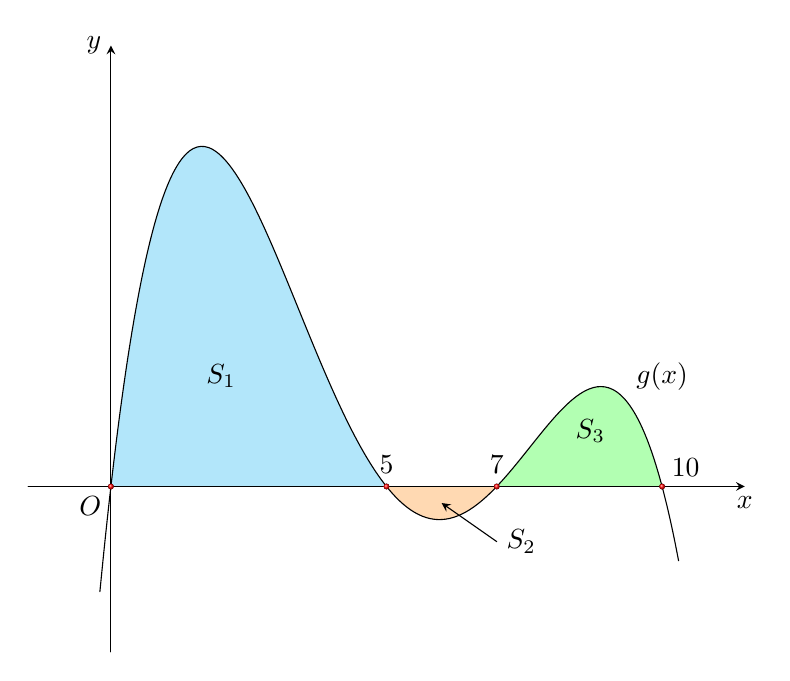
\begin{tikzpicture}[line join=round,line cap=round,>=stealth,scale=0.7,declare function={g (\x) = -0.5*\x*(\x-5)*(\x-7)*(\x-10);}]
			\begin{scope}[yscale=0.05]
				\fill[cyan,opacity=0.3] (0,0)--plot[samples=150,smooth,domain=0:5] (\x,{g (\x)})--(5,0)--cycle;
				\fill[orange,opacity=0.3] (5,0)--plot[samples=150,smooth,domain=5:7] (\x,{g (\x)})--(7,0)--cycle;
				\fill[green,opacity=0.3] (7,0)--plot[samples=150,smooth,domain=7:10] (\x,{g (\x)})--(10,0)--cycle;
				\draw plot[samples=150,smooth,domain=-0.2:10.3] (\x,{g (\x)});
			\end{scope}
			\draw[->] (-1.5,0) -- (11.5,0) node[below] {$x$};
			\draw[->] (0,-3) -- (0,8) node[left] {$y$};
			\node at (0,0) [below left] {$O$};
			\foreach \diem in {(0,0),(5,0),(7,0),(10,0)}{\fill[ball color=red] \diem circle (1.5pt);}
			\node[above=1pt] at (5,0) {$5$};
			\node[above=1pt] at (7,0) {$7$};
			\node[above right] at (10,0) {$10$};
			\node at (2,2) {$S_1$};
			\node at (8.7,1) {$S_3$};
			\draw[<-] (6,-0.3)--(7,-1) node[right] {$S_2$};
			\node at (10,2) {$g (x)$};
		\end{tikzpicture}
	\end{center}
	\choiceTF
	{\True $S_1 = f(5)$}
	{$S_2 = f(7) - f(5)$}
	{\True $f(5) > f(7)$}
	{\True $f(10) > f(5)$}
	\loigiai{
		Theo định nghĩa, ta có $f(0) = \displaystyle\int\limits_{0}^{0} g(t)\mathrm{\,d}t = 0$.
		\begin{itemchoice}
			\itemch Do trên đoạn $[0;5]$, đồ thị nằm trên trục hoành nên $g(x) \ge 0$. \\
			Ta có $S_1 = \displaystyle\int\limits_{0}^{5} |g(t)|\mathrm{\,d}t = \displaystyle\int\limits_{0}^{5} g(t)\mathrm{\,d}t = f(5) - f(0) = f(5)$.
			\itemch Do trên đoạn $[5;7]$, đồ thị nằm dưới trục hoành nên $g(x) \le 0$. \\
			Ta có $S_2 = \displaystyle\int\limits_{5}^{7} |g(t)|\mathrm{\,d}t = -\displaystyle\int\limits_{5}^{7} g(t)\mathrm{\,d}t = -\left( f(7) - f(5) \right) = f(5) - f(7)$.
			\itemch Theo chứng minh trên ta có $S_2 = f(5) - f(7)$. \\
			Mà diện tích $S_2 > 0$ nên $f(5) - f(7) > 0 \Leftrightarrow f(5) > f(7)$.
			\itemch Trên đoạn $[7;10]$, đồ thị nằm trên trục hoành nên $g(x) \ge 0$. \\
			Ta có $S_3 = \displaystyle\int\limits_{7}^{10} |g(t)|\mathrm{\,d}t = \displaystyle\int\limits_{7}^{10} g(t)\mathrm{\,d}t = f(10) - f(7)$.\\
			Suy ra $f(10) = f(7) + S_3 = (f(5) - S_2) + S_3 = f(5) + (S_3 - S_2)$.\\
			Dựa vào đồ thị và hàm số $g(x)$, diện tích $S_3$ lớn hơn phần diện tích $S_2$, tức là $S_3 - S_2 > 0$.\\
			Do đó $f(10) > f(5)$.
		\end{itemchoice}
	}
\end{ex}
%%%=============================%%%

%%%=============EX_15=============%%%
\begin{ex}%[2D6V2-4]%[TBMZZ14]%[Vũ Hồng Toàn]
	Một doanh nghiệp dự định sản xuất $10\,000$ sản phẩm một loại mặt hàng và chia thành hai phần $4\,000$, $6\,000$ sản phẩm để chia ngẫu nhiên cho hai xí nghiệp I, II sản xuất. Tỉ lệ phế phẩm của các xí nghiệp I, II lần lượt là $3\%$, $5\%$. Tiến hành tung một con xúc sắc cân đối đồng chất, nếu số chấm nhỏ hơn $5$ thì giao cho xí nghiệp I sản xuất $6\,000$ sản phẩm và nếu số chấm lớn hơn $4$ thì giao cho xí nghiệp I sản xuất $4\,000$ sản phẩm. Chọn ngẫu nhiên một sản phẩm từ doanh nghiệp. Gọi $A$ là biến cố xí nghiệp I sản xuất $6\,000$ sản phẩm, $B$ là biến cố chọn được sản phẩm của xí nghiệp I, $C$ là biến cố chọn được sản phẩm là phế phẩm.
	\choiceTF
	{\True $\mathrm{P}(A) = \dfrac{2}{3}$}
	{$\mathrm{P}(B) = \dfrac{4}{15}$}
	{$\mathrm{P}(C) = \dfrac{59}{1\,505}$}
	{$\mathrm{P}(C\mid A) = \dfrac{19}{400}$}
	\loigiai{
		Từ giả thiết, ta có sơ đồ hình cây như sau:
		\begin{center}
			\begin{tikzpicture}[declare function={dai=2.8;cao=0.7;},>=stealth,font=\scriptsize]
				\tikzset{nhan/.style={minimum size=19pt,font=\small,inner sep=2pt}}
				
				% Các điểm nút (Nodes)
				\path (0,0) node[nhan] (G){\textbf{Gốc}}
				
				% Cấp 1: Biến cố A (Tung xúc sắc)
				(dai,{4*cao}) node[nhan] (A) {$A$}
				(dai,{-4*cao}) node[nhan] (nA) {$\overline{A}$}
				
				% Cấp 2: Biến cố B (Chọn sản phẩm của XN I hay II)
				({2*dai},{6*cao}) node[nhan] (AB) {$B$}
				({2*dai},{2*cao}) node[nhan] (AnB) {$\overline{B}$}
				({2*dai},{-2*cao}) node[nhan] (nAB) {$B$}
				({2*dai},{-6*cao}) node[nhan] (nAnB) {$\overline{B}$}
				
				% Cấp 3: Biến cố C (Kiểm tra phế phẩm)
				({3*dai},{7*cao}) node[nhan] (ABC) {$C$}
				({3*dai},{5*cao}) node[nhan] (ABCn) {$\overline{C}$}
				({3*dai},{3*cao}) node[nhan] (AnBC) {$C$}
				({3*dai},{cao}) node[nhan] (AnBCn) {$\overline{C}$}
				({3*dai},{-cao}) node[nhan] (nABC) {$C$}
				({3*dai},{-3*cao}) node[nhan] (nABCn) {$\overline{C}$}
				({3*dai},{-5*cao}) node[nhan] (nAnBC) {$C$}
				({3*dai},{-7*cao}) node[nhan] (nAnBCn) {$\overline{C}$};
				
				% Vẽ các mũi tên và ghi chú xác suất
				% Nhánh từ Gốc đến A
				\draw[->] (G.east) -- (A.west) node[sloped,pos=0.5,above]{$2/3$};
				\draw[->] (G.east) -- (nA.west) node[sloped,pos=0.5,below]{$1/3$};
				
				% Nhánh từ A đến B
				\draw[->] (A.east) -- (AB.west) node[sloped,pos=0.5,above]{$0{,}6$};
				\draw[->] (A.east) -- (AnB.west) node[sloped,pos=0.5,below]{$0{,}4$};
				
				% Nhánh từ non-A đến B
				\draw[->] (nA.east) -- (nAB.west) node[sloped,pos=0.5,above]{$0{,}4$};
				\draw[->] (nA.east) -- (nAnB.west) node[sloped,pos=0.5,below]{$0{,}6$};
				
				% Nhánh phế phẩm (C) cho XN I (B)
				\draw[->] (AB.east) -- (ABC.west) node[sloped,pos=0.5,above]{$0{,}03$};
				\draw[->] (AB.east) -- (ABCn.west) node[sloped,pos=0.5,below]{$0{,}97$};
				
				\draw[->] (nAB.east) -- (nABC.west) node[sloped,pos=0.5,above]{$0{,}03$};
				\draw[->] (nAB.east) -- (nABCn.west) node[sloped,pos=0.5,below]{$0{,}97$};
				
				% Nhánh phế phẩm (C) cho XN II (non-B)
				\draw[->] (AnB.east) -- (AnBC.west) node[sloped,pos=0.5,above]{$0{,}05$};
				\draw[->] (AnB.east) -- (AnBCn.west) node[sloped,pos=0.5,below]{$0{,}95$};
				
				\draw[->] (nAnB.east) -- (nAnBC.west) node[sloped,pos=0.5,above]{$0{,}05$};
				\draw[->] (nAnB.east) -- (nAnBCn.west) node[sloped,pos=0.5,below]{$0{,}95$};
			\end{tikzpicture}
		\end{center}
		\begin{itemchoice}
			\itemch Xét biến cố $A$: \lq\lq Xí nghiệp I sản xuất $6\,000$ sản phẩm\rq\rq.\\ 
			Biến cố này xảy ra khi tung xúc sắc được số chấm nhỏ hơn $5$, tức là các mặt $\{1; 2; 3; 4\}$. \\
			Do đó, $\mathrm{P}(A) = \dfrac{4}{6} = \dfrac{2}{3}$.
			\itemch Xét biến cố $B$: \lq\lq Chọn được sản phẩm của xí nghiệp I\rq\rq.
			\begin{itemize}
				\item Nếu $A$ xảy ra ($\mathrm{P}(A) = \dfrac{2}{3}$), xí nghiệp I sản xuất $6\,000$ sản phẩm trên tổng số $10\,000$ sản phẩm nên $\mathrm{P}(B \mid A) = \dfrac{6\,000}{10\,000} = \dfrac{3}{5}$.
				\item Nếu $\overline{A}$ xảy ra ($\mathrm{P}(\overline{A}) = 1 - \dfrac{2}{3} = \dfrac{1}{3}$), xí nghiệp I sản xuất $4\,000$ sản phẩm nên $\mathrm{P}(B \mid \overline{A}) = \dfrac{4\,000}{10\,000} = \dfrac{2}{5}$.
			\end{itemize}
			Theo công thức xác suất toàn phần, ta có
			\[\mathrm{P}(B) = \mathrm{P}(A) \cdot \mathrm{P}(B \mid A) + \mathrm{P}(\overline{A}) \cdot \mathrm{P}(B \mid \overline{A}) = \dfrac{2}{3} \cdot \dfrac{3}{5} + \dfrac{1}{3} \cdot \dfrac{2}{5} = \dfrac{8}{15}.\]
			\itemch Xét biến cố $C$: \lq\lq Chọn được sản phẩm là phế phẩm\rq\rq. \\
			Gọi $I$ là biến cố sản phẩm thuộc xí nghiệp I, $II$ là biến cố sản phẩm thuộc xí nghiệp II. Ta có $\mathrm{P}(I) = \mathrm{P}(B) = \dfrac{8}{15}$ và $\mathrm{P}(II) = 1 - \mathrm{P}(B) = \dfrac{7}{15}$. \\
			Tỉ lệ phế phẩm của xí nghiệp I là $3\%$, xí nghiệp II là $5\%$.\\
			Do đó
			\[\mathrm{P}(C) = \mathrm{P}(I) \cdot 3\% + \mathrm{P}(II) \cdot 5\% = \dfrac{8}{15} \cdot \dfrac{3}{100} + \dfrac{7}{15} \cdot \dfrac{5}{100} = \dfrac{59}{1\,500}.\]
			\itemch Khi biến cố $A$ xảy ra, xí nghiệp I sản xuất $6\,000$ sản phẩm (có $6\,000 \cdot 3\% = 180$ phế phẩm) và xí nghiệp II sản xuất $4\,000$ sản phẩm (có $4\,000 \cdot 5\% = 200$ phế phẩm). \\
			Tổng số phế phẩm trong $10\,000$ sản phẩm lúc này là $180 + 200 = 380$.\\ 
			Khi đó
			\[\mathrm{P}(C \mid A) = \dfrac{380}{10\,000} = \dfrac{19}{500}.\]
		\end{itemchoice}
	}
\end{ex}
%%%=============================%%%

%%%=============EX_16=============%%%
\begin{ex} %[2H5V2-8]%[TDMZZ14]%[Hà Văn Hảo]
	Trong không gian $Oxyz$ có đơn vị dài trên mỗi trục là centimet, có một thanh cứng ở thời điểm ban đầu $t_0 = 0$ có hai đầu ở các vị trí $A(0;0;0)$, $B(40;20;0)$ và có một sợi dây căng đủ dài nằm trên đường thẳng $d \colon \heva{&x = 30 + 2t \\ &y = 25 + 3t \\ &z = 40}$. Thanh cứng này bắt đầu chuyển động tịnh tiến với tốc độ bằng $18$\,cm/s theo hướng vectơ $\overrightarrow{u} = (1;2;2)$.
	\choiceTF
	{\True Phương trình tham số của đường thẳng $AB$ là $\heva{&x = 2t' \\ &y = t' \\ &z = 0}$, $t' \in \mathbb{R}$}
	{Thanh cứng va chạm vào dây $d$ tại điểm $N(30 + 2t; 25 + 35t; 40)$ với $t \in \mathbb{R}$}
	{\True Gọi $M$ là vị trí ban đầu của điểm trên thanh cứng va chạm vào dây $d$. Khi đó ta có $\overrightarrow{MN} = k\overrightarrow{u}$, $k \in \mathbb{R}$, $k \ge 0$ với $t \in \mathbb{R}$}
	{Thời điểm mà thanh cứng va chạm vào dây $t = 21{,}4$ giây (\textit{tính theo đơn vị giây và làm tròn kết quả đến hàng phần mười})}
	\loigiai{
		\begin{itemchoice}
			\itemch Vectơ chỉ phương của đường thẳng $AB$ là $\overrightarrow{AB} = (40;20;0) = 20(2;1;0)$.\\
			Đường thẳng $AB$ đi qua gốc tọa độ $A(0;0;0)$ có phương trình tham số là $\heva{&x = 2t' \\ &y = t' \\ &z = 0.}$
			\itemch Vì điểm va chạm $N$ nằm trên dây $d$ nên có tọa độ $N(30 + 2t; 25 + 3t; 40)$.
			\itemch Vì thanh chuyển động tịnh tiến theo hướng $\overrightarrow{u}$, mọi điểm trên thanh đều di chuyển theo các đường thẳng song song hoặc trùng với giá của $\overrightarrow{u}$.\\
			Do đó, vectơ dịch chuyển $\overrightarrow{MN}$ phải cùng hướng với $\overrightarrow{u}$, tức là $\overrightarrow{MN} = k\overrightarrow{u}$ với $k \ge 0$.
			\itemch Gọi $M(2t'; t'; 0)$ là một điểm bất kỳ thuộc thanh $AB$ ($0 \le 2t' \le 40 \Rightarrow 0 \le t' \le 20$).\\
			Vectơ vận tốc $\overrightarrow{v}$ có độ lớn $18$\,cm/s và cùng hướng với $\overrightarrow{u} = (1;2;2)$.\\
			Ta có $|\overrightarrow{u}| = \sqrt{1^2 + 2^2 + 2^2} = 3$. \\
			Vectơ vận tốc là $\overrightarrow{v} = \dfrac{18}{|\overrightarrow{u}|} \cdot \overrightarrow{u} = \dfrac{18}{3}(1;2;2) = (6; 12; 12)$.\\
			Tọa độ điểm $M$ sau thời gian $T$ giây là $M_T = (2t' + 6T; t' + 12T; 12T)$.\\
			Để thanh va chạm với dây $d$, tồn tại thời điểm $T$ và giá trị $t, t'$ sao cho $M_T \equiv N \in d$. \\
			Do đó
			$\heva{&2t' + 6T = 30 + 2t & (1)\\ &t' + 12T = 25 + 3t & (2)\\ &12T = 40 & (3).}$\\
			Từ (3) suy ra $T = \dfrac{40}{12} = \dfrac{10}{3} \approx 3{,}3$ (s). \\
			Thay $T = \dfrac{10}{3}$ vào (1) và (2) ta có hệ phương trình
			$\heva{&2t' - 2t = 10 \\ &t' - 3t = -15}$. \\
			Giải hệ ta được $t = 10$ và $t' = 15 \in [0; 20]$ (thỏa mãn $M$ nằm trên thanh $AB$).\\
			Vậy thời điểm va chạm là $T \approx 3{,}3 \text{ (s)}$.
		\end{itemchoice}
	}
\end{ex}
%%%=============================%%%

\caukq
%%%=============EX_17=============%%%
\begin{ex}%[1H8V6-2]%[TDMZZ11]%[Duong Xuan Loi]
	Cho hình chóp $S.ABCD$ có đáy là hình vuông cạnh bằng $6$, cạnh bên $SA$ vuông góc với đáy và có $SA=8$. Hãy xác định số đo góc nhị diện $[S,BD,C]$ theo đơn vị độ (\textit{làm tròn kết quả đến hàng đơn vị}).
	\par
	\shortans[0]{118}
	\loigiai{
		\begin{center}
			\begin{tikzpicture}[scale=1, font=\footnotesize, line join=round, line cap=round,>=stealth]
				\path
				(0,0) coordinate (A)
				(-1.3,-1.6) coordinate (B)
				(2.5,-1.6)coordinate (C)
				($(A)+(C)-(B)$) coordinate (D)
				($(A)+(0,3)$) coordinate (S)
				(intersection of A--C and B--D) coordinate (O)
				;
				\draw (S)--(B)--(C)--(D)--cycle (S)--(C);
				\draw[dashed] (O)--(S)--(A)--(D) (C)--(A)--(B)--(D);	
				\foreach \p/\q in {S/90,A/-90,B/-90,C/-90,D/0,O/-90}			
				\fill[black] (\p) circle (1.0pt)node[shift={(\q:2.5mm)}]{$\p$};
				\draw pic[draw=black,angle radius=0.2cm] {right angle = S--A--B}; 
				\draw pic[draw=black,angle radius=0.2cm] {right angle = S--A--D}; 
			\end{tikzpicture}
		\end{center}
		Gọi $O$ là giao điểm của hai đường chéo $AC$ và $BD$.\\
		Vì $ABCD$ là hình vuông nên $BD \perp AC$ tại trung điểm $O$.\\
		Vì $SA \perp (ABCD)$ nên $SA \perp BD$.\\
		Từ $BD \perp AC$ và $BD \perp SA$ suy ra $BD \perp (SAC)$.\\
		Do $SO \subset (SAC)$ và $AO \subset (SAC)$ nên $BD \perp SO$ và $BD \perp AO$.\\
		Suy ra góc phẳng nhị diện $[S,BD,A]$ chính là góc $\widehat{SOA}$.\\
		Hình vuông $ABCD$ có cạnh bằng $6$ nên đường chéo $AC = 6\sqrt{2} \Rightarrow OA = \dfrac{AC}{2} = 3\sqrt{2}$.\\
		Xét tam giác $SAO$ vuông tại $A$, ta tính được $\tan \widehat{SOA} = \dfrac{SA}{OA} = \dfrac{8}{3\sqrt{2}} = \dfrac{4\sqrt{2}}{3}\Rightarrow \widehat{SOA} \approx 62{,}06^\circ$.\\
		Do ba điểm $A$, $O$, $C$ thẳng hàng và $O$ nằm giữa $A$ và $C$ nên hai góc nhị diện $[S,BD,A]$ và $[S,BD,C]$ là hai góc kề bù.\\
		Suy ra số đo góc nhị diện $[S,BD,C]$ là $\widehat{SOC} = 180^\circ - \widehat{SOA} \approx 180^\circ - 62{,}06^\circ = 117{,}94^\circ \approx 118^\circ$.
	}
\end{ex}
%%%=============================%%%

%%%=============EX_18=============%%%
\begin{ex}%[2D1H3-6]%[TDMZZ14]%[Lê Minh]
	Một hộ sản xuất chuyên làm thịt bò khô để bán, mỗi ngày hộ đó sản xuất được $x$\,kg thịt bò khô ($1 \le x \le 30$). Tổng chi phí sản xuất $x$\,kg thịt bò khô tính bằng nghìn đồng, cho bởi hàm chi phí $C(x) = x^3 - 9x^2 + 480x + 600$. Giả sử hộ gia đình này luôn bán hết số thịt làm ra mỗi ngày với giá $780$ nghìn đồng/kg. Hỏi lợi nhuận tối đa mà hộ gia đình này thu được từ việc sản xuất và bán thịt bò khô trong một ngày là bao nhiêu nghìn đồng \textit{(không làm tròn các phép tính trung gian và kết quả cuối cùng được làm tròn đến hàng đơn vị)}?
	\par
	\shortans[0]{2630}
	\loigiai{
		Doanh thu khi bán $x$\,kg thịt bò khô là $R(x) = 780x$ (nghìn đồng). \\
		Lợi nhuận thu được trong một ngày là 
		\[L(x) = R(x) - C(x) = 780x - \left(x^3 - 9x^2 + 480x + 600\right) = -x^3 + 9x^2 + 300x - 600.\]
		Ta có $L'(x) = -3x^2 + 18x + 300$. \\
		Khi đó $L'(x) = 0 \Leftrightarrow -3x^2 + 18x + 300 = 0 \Leftrightarrow x^2 - 6x - 100 = 0 \Leftrightarrow \hoac{&x = 3+\sqrt{109} \in [1; 30] \\ &x = 3-\sqrt{109} \notin [1; 30].}$ \\
		Ta đi tính giá trị của hàm số tại các điểm biên và điểm cực trị:\\
		Ta có $L(1) = -1 + 9 + 300 - 600 = -292$.\\
		$L(30) = -30^3 + 9\cdot 30^2 + 300\cdot 30 - 600 = -10\,500$.\\
		Để tính chính xác $L\left(3+\sqrt{109}\right)$, ta thực hiện phép chia đa thức $L(x)$ cho $L'(x)$:
		\begin{align*}
			L(x) &= -x(x^2) + 9x^2 + 300x - 600 = -x(6x+100) + 9x^2 + 300x - 600 \\
			&= 3x^2 + 200x - 600 = 3(6x+100) + 200x - 600 = 218x - 300.
		\end{align*}
		Thay $x = 3+\sqrt{109}$ vào ta được
		\[ L\left(3+\sqrt{109}\right) = 218\left(3+\sqrt{109}\right) - 300 = 354 + 218\sqrt{109} \approx 2\,630{,}14. \]
		Bảng biến thiên của hàm số $L(x)$ trên đoạn $[1; 30]$:
		\begin{center}
			
\begin{tikzpicture}
				\tkzTabInit[nocadre=true, lgt=1.2, espcl=4, deltacl=0.65]
				{$x$/1.0, $L'(x)$/0.7, $L(x)$/2}
				{$1$, $3+\sqrt{109}$, $30$}
				\tkzTabLine{,+,0,-,}
				\tkzTabVar{-/ $-292$, +/ $354+218\sqrt{109}$, -/ $-10\,500$}
			\end{tikzpicture}
		\end{center}
		Vậy lợi nhuận tối đa của hộ gia đình xấp xỉ $2\,630$ nghìn đồng.
	}
\end{ex}
%%%=============================%%%

%%%=============EX_19=============%%%
\begin{ex}%[2H5V3-4]%[TDMZZ14-19-TLN]%[Nguyễn Văn Sang]
	Trong không gian $Oxyz$ có đơn vị dài trên mỗi trục là centimet, cho một quả cầu $(S)$ có bán kính bằng $30$\,cm, ở thời điểm ban đầu $t_0 = 0$ có tọa độ tâm là $I_0(20;10;0)$ và hai điểm cố định trong không gian có tọa độ $A(25;56;9)$, $B(21;59;24)$.
	Quả cầu $(S)$ bắt đầu chuyển động tịnh tiến theo hướng véctơ $\overrightarrow{u}=(0;3;2)$ với tốc độ $8$\,cm/s. Biết rằng quả cầu bị dừng lại ngay khi va chạm vào một trong hai điểm $A$ hoặc $B$. Hãy tính theo đơn vị giây thời điểm mà quả cầu này bị dừng lại (\textit{không làm tròn các phép tính trung gian và kết quả cuối cùng được làm tròn đến hàng phần trăm}).
	\begin{center}
		\begin{tikzpicture}[scale=0.9, >=stealth]
			% Định nghĩa bán kính R trên hình vẽ
			\def\R{2.2}
			
			% Các điểm chuẩn
			\coordinate (I0) at (0,0);
			\coordinate (IA) at (7,2.5); % Tâm quả cầu khi chạm A
			
			% Véctơ hướng chuyển động (kéo dài qua IA)
			\coordinate (Dir) at (6, 3.57); 
			
			% Điểm A nằm chính xác trên bề mặt khối cầu mờ tại I_A
			\coordinate (A) at ($(IA) + (25: \R)$);
			% Điểm B nằm ngoài đường di chuyển
			\coordinate (B) at (8, 5.5);
			
			% Vẽ quỹ đạo tịnh tiến
			\draw[dashed, thick, violet, ->] (I0) -- (Dir) node[above] {Hướng tịnh tiến $\overrightarrow{u}$};
			
			% --- Vẽ quả cầu tại vị trí xuất phát I_0 ---
			% Đổ bóng khối cầu
			\shade[ball color=cyan!30, opacity=0.8] (I0) circle (\R);
			\draw[cyan!80!blue, thick] (I0) circle (\R);
			
			% Vĩ tuyến (Equator) - Trước liền, sau đứt
			\draw[cyan!70!blue, thin] (-\R,0) arc (180:360:{\R} and {0.3*\R});
			\draw[cyan!70!blue, dashed, thin] (\R,0) arc (0:180:{\R} and {0.3*\R});
			
			% Kinh tuyến (Meridian) - Trước liền, sau đứt
			\draw[cyan!70!blue, thin] (0,-\R) arc (-90:90:{0.3*\R} and {\R});
			\draw[cyan!70!blue, dashed, thin] (0,\R) arc (90:270:{0.3*\R} and {\R});
			
			% Điểm tâm I_0
			\fill[black] (I0) circle (2pt) node[below left] {$I_0$};
			\fill[red] (A) circle (2.5pt) node[right, red] {$A$};
			\fill[blue] (B) circle (2.5pt) node[right, blue] {$B$};
		\end{tikzpicture}
	\end{center}
	\par
	\shortans[0]{2,48}
	\loigiai{
		\begin{center}
			\begin{tikzpicture}[scale=0.9, >=stealth]
				% Định nghĩa bán kính R trên hình vẽ
				\def\R{2.2}
				
				% Các điểm chuẩn
				\coordinate (I0) at (0,0);
				\coordinate (IA) at (7,2.5); % Tâm quả cầu khi chạm A
				
				% Véctơ hướng chuyển động (kéo dài qua IA)
				\coordinate (Dir) at (10, 3.57); 
				
				% Điểm A nằm chính xác trên bề mặt khối cầu mờ tại I_A
				\coordinate (A) at ($(IA) + (25: \R)$);
				% Điểm B nằm ngoài đường di chuyển
				\coordinate (B) at (8, 5.5);
				
				% Vẽ quỹ đạo tịnh tiến
				\draw[dashed, thick, violet, ->] (I0) -- (Dir) node[right] {Hướng tịnh tiến $\overrightarrow{u}$};
				
				% --- Vẽ quả cầu tại vị trí xuất phát I_0 ---
				% Đổ bóng khối cầu
				\shade[ball color=cyan!30, opacity=0.8] (I0) circle (\R);
				\draw[cyan!80!blue, thick] (I0) circle (\R);
				
				% Vĩ tuyến (Equator) - Trước liền, sau đứt
				\draw[cyan!70!blue, thin] (-\R,0) arc (180:360:{\R} and {0.3*\R});
				\draw[cyan!70!blue, dashed, thin] (\R,0) arc (0:180:{\R} and {0.3*\R});
				
				% Kinh tuyến (Meridian) - Trước liền, sau đứt
				\draw[cyan!70!blue, thin] (0,-\R) arc (-90:90:{0.3*\R} and {\R});
				\draw[cyan!70!blue, dashed, thin] (0,\R) arc (90:270:{0.3*\R} and {\R});
				
				% Điểm tâm I_0
				\fill[black] (I0) circle (2pt) node[below left] {$I_0$};
				
				% --- Vẽ bóng mờ quả cầu tại vị trí dừng lại I_A ---
				\draw[cyan!50!blue, dashed, thick] (IA) circle (\R);
				\shade[ball color=cyan!10, opacity=0.25] (IA) circle (\R);
				
				% Điểm tâm I_A
				\fill[black!70] (IA) circle (2pt) node[above left, black] {$I_A$};
				
				% Bán kính nối từ I_A đến bề mặt chạm A
				\draw[thick, red, ->] (IA) -- (A) node[midway, sloped, above] {$R=30$};
				
				% Chấm điểm A và B
				\fill[red] (A) circle (2.5pt) node[right, red] {$A$};
				\fill[blue] (B) circle (2.5pt) node[right, blue] {$B$};
				
				% Chú thích mô phỏng
				\node[align=center, below, text=black!70] at (3.5, -2.5) {\textit{Mô phỏng: Quả cầu tịnh tiến từ $I_0$}\\ \textit{và dừng lại khi bề mặt chạm điểm $A$}};
			\end{tikzpicture}
		\end{center}
		Ta có hướng di chuyển của quả cầu là véctơ $\overrightarrow{u} = (0;3;2) \Rightarrow |\overrightarrow{u}| = \sqrt{0^2 + 3^2 + 2^2} = \sqrt{13}$.\\
		Vì tốc độ của quả cầu là $v = 8$\,cm/s nên véctơ vận tốc của quả cầu là
		$\overrightarrow{v} = 8 \cdot \dfrac{\overrightarrow{u}}{|\overrightarrow{u}|} = \left( 0 ; \dfrac{24}{\sqrt{13}} ; \dfrac{16}{\sqrt{13}} \right)$.\\
		Tọa độ tâm $I$ của quả cầu tại thời điểm $t$ ($t \ge 0$) là
		$ \heva{& x_I = 20 \\ & y_I = 10 + \dfrac{24}{\sqrt{13}}t \\ & z_I = 0 + \dfrac{16}{\sqrt{13}}t.}$\\
		Đặt $k = \dfrac{8t}{\sqrt{13}}$ ($k \ge 0$). Khi đó, tọa độ tâm $I$ theo biến $k$ là $I(20; 10 + 3k; 2k)$.
		\begin{enumerate}[\it TH 1:]
			\item \textbf{Kiểm tra va chạm với điểm $A(25; 56; 9)$.}\\
			Quả cầu chạm điểm $A$ khi $IA^2 = R^2 = 30^2 = 900$.
			\allowdisplaybreaks
			\begin{eqnarray*}
				&& (25 - 20)^2 + \big[56 - (10 + 3k)\big]^2 + (9 - 2k)^2 = 900\\
				&\Leftrightarrow& 13k^2 - 312k + 1322 = 0\\
				&\Leftrightarrow& k=\dfrac{156 \pm 5\sqrt{286}}{13}.
			\end{eqnarray*}
			Vì quả cầu lao về phía điểm $A$ và sẽ dừng lại ở lần chạm đầu tiên (bề mặt ngoài), ta chọn nghiệm nhỏ hơn
			\[ k_A = \dfrac{156 - 5\sqrt{286}}{13} \approx 5{,}495. \]
			\item \textbf{Kiểm tra va chạm với điểm $B(21; 59; 24)$.}\\
			Quả cầu chạm điểm $B$ khi $IB^2 = R^2 = 900$.
			\begin{eqnarray*}
				&& (21 - 20)^2 + \big[59 - (10 + 3k)\big]^2 + (24 - 2k)^2 = 900\\
				&\Leftrightarrow& 13k^2 - 390k + 2078 = 0\\
				&\Leftrightarrow& k = \dfrac{195 \pm \sqrt{11011}}{13}.
			\end{eqnarray*}
			Ta lấy nghiệm nhỏ hơn cho lần chạm đầu tiên
			\[ k_B = \dfrac{195 - \sqrt{11011}}{13} \approx 6{,}928.\]
		\end{enumerate}
		\textbf{Kết luận thời điểm va chạm:} \\
		So sánh hai giá trị $k$, ta thấy $k_A < k_B$. Nghĩa là quả cầu sẽ va chạm vào điểm $A$ trước và dừng lại ngay tại đó, không tiến đến điểm $B$.\\
		Thời gian $t$ ứng với $k_A$ là
		\[ t = \dfrac{k_A \cdot \sqrt{13}}{8} = \dfrac{\sqrt{13}}{8} \cdot \dfrac{156 - 5\sqrt{286}}{13} \approx 2{,}48 \text{ (giây)}. \]
	}
\end{ex}
%%%=============================%%%

%%%=============EX_20=============%%%
\begin{ex}%[2D4C3-4]%[TDMZZ14]%[Trương Tường]
	\immini[thm]{
		Trên một mảnh đất hình vuông $ABCD$ có cạnh bằng $20$ mét người ta muốn trồng hoa trong phần tô màu được giới hạn bởi hai đường parabol bằng nhau và cạnh $CD$. Hãy tính diện tích phần tô màu theo đơn vị mét vuông (\textit{không làm tròn các phép tính trung gian và kết quả cuối cùng được làm tròn đến hàng phần mười}).
	}{
		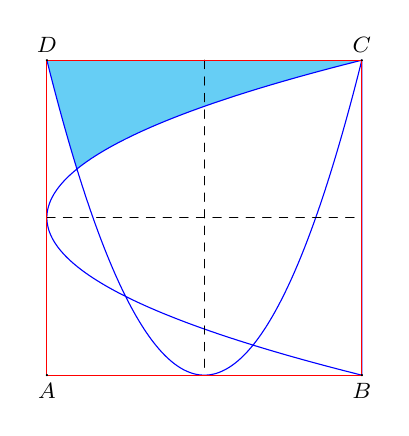
\begin{tikzpicture}[scale=.2, >=stealth, line join=round, line cap=round, font=\footnotesize]
			\tikzset{declare function={f(\x)=.2*(\x)^2-10;x4=(-5-5*sqrt(5))/2;}}
			\path (-10,-10) coordinate (A)
			(10,-10) coordinate (B)
			(10,10) coordinate (C)
			(-10,10) coordinate (D);
			\begin{scope}
				\fill[samples=80, cyan!60]
				plot [domain={-10}:{x4}] ({\x},{f(\x)})--plot [domain={f(x4)}:{f(10)}] ({f(\x)},{\x})--cycle;
			\end{scope}
			\draw[smooth, samples=100, blue] 
			plot[domain=-10:10] ({\x},{f(\x)})
			--plot[domain={-10}:{10}] ({f(\x)},{\x});
			\draw [dashed] (0,10)--(0,-10) (-10,0)--(10,0);
			\draw[red] (A)--(B)--(C)--(D)--cycle;
			\foreach \x/\y in {A/-90, B/-90, C/90, D/90}{
				\draw [fill=black] (\x) circle (1pt) ++(\y:1) node {$\x$};
			}
		\end{tikzpicture}
	}
	\par
	\shortans[0]{58,3}
	\loigiai{
		Chọn hệ trục tọa độ $Oxy$ như hình vẽ dưới đây (đơn vị trên mỗi trục là mét).
		\begin{center}
			\begin{tikzpicture}[scale=.25, >=stealth, line join=round, line cap=round, font=\footnotesize]
				\tikzset{declare function={f(\x)=.2*(\x)^2-10;x4=(-5-5*sqrt(5))/2;x2=(-5+5*sqrt(5))/2;x3=-5;}}
				\def\xmin{-14} \def\xmax{14} \def\ymin{-14} \def\ymax{14} 
				\clip (\xmin,\ymin) rectangle (\xmax,\ymax);
				\path (-10,-10) coordinate (A)
				(10,-10) coordinate (B)
				(10,10) coordinate (C)
				(-10,10) coordinate (D);
				\begin{scope}
					\fill[samples=80, pattern=north east lines]
					plot [domain={-10}:{x4}] ({\x},{f(\x)})--(x4,10)--cycle;
					\fill[samples=80, pattern=horizontal lines]
					plot [domain={f(x4)}:{f(10)}] ({f(\x)},{\x})--(10,10)--(x4,10)--cycle;
				\end{scope}
				\draw[smooth, samples=100, blue] plot[domain=-10:10] ({\x},{f(\x)});
				\draw[smooth, samples=100, violet] plot[domain={-10}:{10}] ({f(\x)},{\x});
				\draw [dashed] (\xmin,\ymin)--(\xmax,\ymax)
				(x2,{f(x2)})--(x2,0) (x3,{f(x3)})--(x3,0)
				;
				\draw[semithick, red] (A)--(B)--(C)--(D)--cycle;
				\draw (x4,\ymin)--(x4,\ymax) node [below right] {$x=x_2$};
				\draw [->] (\xmin,0)--(\xmax,0) node [below, xshift=-3pt] {$x$};
				\draw [->] (0,\ymin)--(0,\ymax) node [left, yshift=-4pt] {$y$};
				\draw [fill=black] (0,0) circle (1pt) node [below right] {$O$}
				(x4,0) circle (1pt) node [below left=0 and -.1] {$x_4$}
				(x2,0) circle (1pt) node [above] {$x_2$}
				(x3,0) circle (1pt) node [above] {$x_3$}
				(x4,{f(x4)}) circle (1pt)
				(x2,{f(x2)}) circle (1pt)
				(x3,{f(x3)}) circle (1pt)
				(-10,0) circle (1pt) node[below left] {$-10$}
				(10,0) circle (1pt) node[below right] {$10$}
				(0,-10) circle (1pt) node[below left] {$-10$}
				(0,10) circle (1pt) node[above left] {$10$}
				;
				\foreach \x/\y in {A/-90, B/-90, C/90, D/90}{
					\draw [fill=black] (\x) circle (1pt) ++(\y:1) node {$\x$};
				}
			\end{tikzpicture}
		\end{center}
		Ta có $A(-10;-10)$, $B(10;-10)$, $C(10;10)$, $D(-10;10)$. \\
		Phương trình đường thẳng $AC$ là $y=x$. \\
		Gọi $(P)$ là parabol đi qua hai điểm $C$ và $D$, $(P')$ là parabol đi qua hai điểm $B$ và $C$. \\
		Parabol $(P)$ có đỉnh $(0;-10)$ thuộc trục tung nên phương trình có dạng $y=f(x)=ax^2+c$. \\
		Ta có hệ phương trình $\heva{&100a+c=10 \\ &c=-10} \Leftrightarrow \heva{&a=0{,}2 \\ &c=-10.}$ \\
		Suy ra $(P) \colon y=f(x)=0{,}2x^2-10$. \\
		Parabol $(P')$ đối xứng với $(P)$ qua đường thẳng $AC \colon y=x$ nên có phương trình
		\[x=0{,}2y^2-10 \Leftrightarrow \hoac{&y=\sqrt{5x+50} \\ &y=-\sqrt{5x+50}.}\]
		Phần tô màu được giới hạn bởi ba đồ thị hàm số $y=f(x)=0{,}2x^2-10$, $y=g(x)=\sqrt{5x+50}$ và $y=10$. \\
		Xét phương trình $f(x)=g(x) \Leftrightarrow 0{,}2x^2-10=\sqrt{5x+50}$. \\
		Bình phương hai vế ta có
		\begin{eqnarray*}
			&& 0{,}04x^4-4x^2+100=5x+50 \\
			&\Leftrightarrow& 4x^4-400x^2-500x+5\,000=0 \\
			&\Leftrightarrow& 4x^2\left(x^2-100\right)-500(x-10)=0 \\
			&\Leftrightarrow& 4x^2(x-10)(x+10)-500(x-10)=0 \\
			&\Leftrightarrow& (x-10)\left(4x^3+40x^2-500\right)=0 \\
			&\Leftrightarrow& (x-10)(x+5)\left(4x^2+20x-100\right)=0 \\
			&\Leftrightarrow& \hoac{&x_1=10 \\ &x_2=\dfrac{-5+5\sqrt{5}}{2} \\ &x_3=-5 \\ &x_4=\dfrac{-5-5\sqrt{5}}{2}.}
		\end{eqnarray*}
		Ta chia phần tô màu thành hai phần như sau:
		\begin{itemize}
			\item Phần thứ nhất giới hạn bởi hai đồ thị hàm số $y=f(x)$, $y=10$ và hai đường thẳng $x=-10$, $x=x_4$.
			\item Phần thứ hai giới hạn bởi hai đồ thị hàm số $y=g(x)$, $y=10$ và hai đường thẳng $x=x_4$, $x=10$.
		\end{itemize}
		Diện tích phần tô màu là
		\[S=\displaystyle\int\limits_{-10}^{x_4} \big[10-f(x)\big]\mathrm{\,d}x+\displaystyle\int\limits_{x_4}^{10} \big[10-g(x)\big]\mathrm{\,d}x \approx 58{,}3 \text{ (m}^2\text{)}.\]
	}
\end{ex}
%%%=============================%%%

%%%=============EX_21=============%%%
\begin{ex}%[2D6C2-4]%[TDMZZ12]%[Nguyễn Đức Tuấn Anh]
	Ban đầu cho hai hộp bi riêng biệt đựng những viên bi có cùng kích thước và cùng khối lượng. Hộp I đựng $4$ viên bi màu đỏ, $2$ viên bi màu xanh, $1$ viên bi vàng còn hộp II đựng $5$ viên bi màu đỏ và $2$ viên bi màu xanh. Tiến hành lấy ngẫu nhiên hai viên bi ở hộp I bỏ sang hộp II, rồi lấy ngẫu nhiên hai viên bi từ hộp II bỏ về hộp I. Hãy tính xác suất để hộp I vẫn có đủ ba loại bi, nếu biết hai viên bi lấy ra từ hộp II cùng màu (\textit{làm tròn kết quả đến hàng phần trăm}).
	\begin{center}
		\begin{tikzpicture}[scale=1, font=\footnotesize, line join=round, line cap=round, >=stealth]
			\tikzstyle{box} = [draw=gray!60, ultra thick, rounded corners=4mm, fill=cyan!5]
			\tikzstyle{innerbox1} = [draw=white, thick, rounded corners=3mm]
			\tikzstyle{innerbox2} = [draw=gray!30, thick, rounded corners=2mm]
			\tikzstyle{redmarble} = [circle, shading=ball, ball color=red!90!black, minimum size=6mm, circular drop shadow={shadow xshift=0.3ex, shadow yshift=-0.3ex, opacity=0.3}]
			\tikzstyle{bluemarble} = [circle, shading=ball, ball color=cyan, minimum size=6mm, circular drop shadow={shadow xshift=0.3ex, shadow yshift=-0.3ex, opacity=0.3}]
			\tikzstyle{yellowmarble} = [circle, shading=ball, ball color=yellow, minimum size=6mm, circular drop shadow={shadow xshift=0.3ex, shadow yshift=-0.3ex, opacity=0.3}]
			% Hộp I
			\node[above, font=\large] at (-2, 1.2) {Hộp I};
			% Vẽ khay nhựa (nhiều lớp để tạo hiệu ứng 3D thành hộp)
			\draw[box] (-3.8, -1.2) rectangle (-0.2, 1.2);
			\draw[innerbox1] (-3.7, -1.1) rectangle (-0.3, 1.1);
			\draw[innerbox2] (-3.6, -1.0) rectangle (-0.4, 1.0);
			% Các viên bi trong Hộp I 
			\node[bluemarble] at (-2.5, 0.6) {};
			\node[bluemarble] at (-1.6, 0.1) {};
			\node[redmarble] at (-3.1, -0.4) {};
			\node[redmarble] at (-2.3, -0.1) {};
			\node[redmarble] at (-1.6, -0.6) {};
			\node[redmarble] at (-0.8, 0.2) {};
			\node[yellowmarble] at (-0.8, -0.6) {};
			\begin{scope}[shift={(0:2)}]
				% Hộp II
				\node[above, font=\large] at (2, 1.2) {Hộp II};
				% Vẽ khay nhựa
				\draw[box] (0.2, -1.2) rectangle (4, 1.2);
				\draw[innerbox1] (0.3, -1.1) rectangle (3.9, 1.1);
				\draw[innerbox2] (0.4, -1.0) rectangle (3.8, 1.0);
				% Các viên bi trong Hộp II
				\node[redmarble] at (1.1, 0.4) {};
				\node[redmarble] at (1.1, -0.5) {};
				\node[bluemarble] at (1.8, 0.3) {};
				\node[redmarble] at (1.9, -0.6) {};
				\node[bluemarble] at (2.6, -0.2) {};
				\node[redmarble] at (2.7, 0.5) {};
				\node[redmarble] at (3.4, -0.5) {};
			\end{scope}
		\end{tikzpicture}
	\end{center}
	\par
	\shortans[0]{0,74}
	\loigiai{
		Gọi $A$ là biến cố \lq\lq Hộp I vẫn có đủ ba loại bi sau hai lần chuyển\rq\rq.\\
		Gọi $B$ là biến cố \lq\lq Hai viên bi lấy ra từ hộp II để bỏ về hộp I có cùng màu\rq\rq.\\
		Bài toán yêu cầu tính xác suất có điều kiện $\mathrm{P}(A \mid B) = \dfrac{\mathrm{P}(A \cap B)}{\mathrm{P}(B)}$.\\
		\textbf{Xét biến cố $B$:}
		\begin{enumerate}[\it TH 1:]
			\item Lấy $2$ viên bi màu đỏ từ hộp I bỏ sang hộp II. Số cách là $\mathrm{C}_4^2$.\\
			Lúc này hộp II có $7$ đỏ, $2$ xanh. Lấy $2$ viên bi cùng màu từ hộp II bỏ về hộp I, số cách là $\mathrm{C}_7^2 + \mathrm{C}_2^2$.\\
			Trường hợp này có $\mathrm{C}_4^2 \big( \mathrm{C}_7^2 + \mathrm{C}_2^2 \big) = 132$ cách.
			\item Lấy $1$ viên đỏ, $1$ viên xanh từ hộp I bỏ sang hộp II. Số cách là $\mathrm{C}_4^1 \cdot \mathrm{C}_2^1$.\\
			Lúc này hộp II có $6$ đỏ, $3$ xanh. Lấy $2$ viên bi cùng màu từ hộp II bỏ về hộp I, số cách là $\mathrm{C}_6^2 + \mathrm{C}_3^2$.\\
			Trường hợp này có $\mathrm{C}_4^1 \cdot \mathrm{C}_2^1 \big( \mathrm{C}_6^2 + \mathrm{C}_3^2 \big) = 144$ cách.
			\item Lấy $1$ viên đỏ, $1$ viên vàng từ hộp I bỏ sang hộp II. Số cách là $\mathrm{C}_4^1 \cdot \mathrm{C}_1^1$.\\
			Lúc này hộp II có $6$ đỏ, $2$ xanh, $1$ vàng. Lấy $2$ viên bi cùng màu từ hộp II, số cách là $\mathrm{C}_6^2 + \mathrm{C}_2^2$.\\
			Trường hợp này có $\mathrm{C}_4^1 \cdot \mathrm{C}_1^1 \big( \mathrm{C}_6^2 + \mathrm{C}_2^2 \big) = 64$ cách.
			\item Lấy $2$ viên xanh từ hộp I bỏ sang hộp II. Số cách là $\mathrm{C}_2^2$.\\
			Lúc này hộp II có $5$ đỏ, $4$ xanh. Lấy $2$ viên bi cùng màu từ hộp II, số cách là $\mathrm{C}_5^2 + \mathrm{C}_4^2$.\\
			Trường hợp này có $\mathrm{C}_2^2 \big( \mathrm{C}_5^2 + \mathrm{C}_4^2 \big) = 16$ cách.
			\item Lấy $1$ viên xanh, $1$ viên vàng từ hộp I bỏ sang hộp II. Số cách là $\mathrm{C}_2^1 \cdot \mathrm{C}_1^1$.\\
			Lúc này hộp II có $5$ đỏ, $3$ xanh, $1$ vàng. Lấy $2$ viên bi cùng màu từ hộp II, số cách là $\mathrm{C}_5^2 + \mathrm{C}_3^2$.\\
			Trường hợp này có $\mathrm{C}_2^1 \cdot \mathrm{C}_1^1 \big( \mathrm{C}_5^2 + \mathrm{C}_3^2 \big) = 26$ cách.
		\end{enumerate}
		Suy ra $n(B) = 132 + 144 + 64 + 16 + 26 = 382$.\\
		Không gian mẫu của hai phép thử là $n(\Omega) = \mathrm{C}_7^2 \cdot \mathrm{C}_9^2 = 756$.\\
		Xác suất của biến cố $B$ là $\mathrm{P}(B) = \dfrac{382}{756} = \dfrac{191}{378}$.\\
		\textbf{Xét biến cố $A\cap B$:}\\
		Để hộp I còn đủ $3$ loại bi thì viên bi vàng (có duy nhất $1$ viên) không được ở hộp II.\\ Nếu lấy viên bi vàng sang hộp II (thuộc \textit{TH 3} và \textit{TH 5}), để thỏa mãn biến cố $B$ ta phải lấy $2$ viên cùng màu từ hộp II về, nhưng hộp II lúc này chỉ có $1$ viên bi vàng nên không thể lấy $2$ viên vàng để bù lại cho hộp I.\\
		Do đó, các trường hợp này không thỏa mãn biến cố $A$. \\
		Ta chỉ xét các trường hợp không lấy bi vàng sang hộp II ở bước đầu:
		\begin{itemize}
			\item Từ \textit{TH 1}, sau khi chuyển đi $2$ viên đỏ, hộp I còn $2$ đỏ, $2$ xanh, $1$ vàng (đã đủ $3$ màu). \\
			Do đó số cách là $\mathrm{C}_4^2 \big( \mathrm{C}_7^2 + \mathrm{C}_2^2 \big) = 132$.
			\item Từ \textit{TH 2}, sau khi chuyển đi $1$ đỏ và $1$ xanh, hộp I còn $3$ đỏ, $1$ xanh, $1$ vàng (đã đủ $3$ màu).
			Do đó, số cách là $\mathrm{C}_4^1 \cdot \mathrm{C}_2^1 \big( \mathrm{C}_6^2 + \mathrm{C}_3^2 \big) = 144$.
			\item Từ \textit{TH 4}, sau khi chuyển đi $2$ viên xanh, hộp I còn $4$ đỏ, $0$ xanh, $1$ vàng (bị thiếu màu xanh). \\
			Để hộp I đủ $3$ màu, $2$ viên bi lấy về từ hộp II bắt buộc phải là $2$ viên màu xanh.\\
			Số cách chọn $2$ viên xanh từ $4$ viên xanh của hộp II là $\mathrm{C}_4^2$.\\
			Suy ra số cách thỏa mãn là $\mathrm{C}_2^2 \cdot \mathrm{C}_4^2 = 1 \cdot 6 = 6$.
		\end{itemize}
		Suy ra $n(A \cap B) = 132 + 144 + 6 = 282$.\\
		Xác suất của biến cố $A \cap B$ là $\mathrm{P}(A \cap B) = \dfrac{282}{756} = \dfrac{47}{126}$.\\
		Vậy xác suất cần tìm là
		\[ \mathrm{P}(A \mid B) = \dfrac{\mathrm{P}(A \cap B)}{\mathrm{P}(B)} = \dfrac{\dfrac{47}{126}}{\dfrac{191}{378}} = \dfrac{141}{191} \approx 0{,}74. \]
	}
\end{ex}
%%%=============================%%%

%%%=============EX_22=============%%%
\begin{ex}%[1H8V5-6]
	Trong không gian $Oxyz$ có đơn vị dài trên mỗi trục là mét, cho một quả cầu đặc $(S)$ có bán kính bằng $0{,}8$\,m, đang được treo bởi một sợi dây $TA$ dài $60$\,cm, điểm $T$ cách mặt sàn $3$\,m. Người ta muốn giữ cho quả cầu $(S)$ lệch về phía bên trái với sợi dây $TA$ nghiêng một góc $30^\circ$ so với phương thẳng đứng, lúc này sợi dây $TA$ đi qua tâm của quả cầu $(S)$. Để làm điều này người ta dự định dùng một thanh cứng $BC = 40$\,cm luồn vào một lỗ trên quả cầu (lỗ sẽ được tạo ra bởi việc khoan kĩ thuật) để hai đầu mỗi đầu thò ra $4$\,cm để buộc hai sợi dây $BM$, $CN$ vào. Hai sợi dây $BM$, $CN$ (có $M$, $N$ nằm trên mặt sàn) song song với nhau và tạo với mặt đất một góc $60^\circ$. Hãy tính theo đơn vị centimét giá trị nhỏ nhất của tổng chiều dài hai sợi dây $BM$, $CN$ (\textit{không làm tròn các phép tính trung gian và kết quả cuối cùng được làm tròn đến hàng đơn vị}).
	\par
	\shortans[0]{232}
	\loigiai{
		\immini{Đổi đơn vị: $R = 0{,}8$\,m $= 80$\,cm, $TA = 60$\,cm, $T$ cách sàn $300$\,cm.\\
			Gọi $I$ là tâm quả cầu. Vì $T$, $I$, $A$ thẳng hàng và $TA$ là dây treo nên $I$ nằm trên $TA$. Suy ra $IT=IA+TA=140$\,cm.\\
			Gọi $H$ là hình chiếu của $T$ xuống mặt sàn, ta có $TH=300$\,cm và $\widehat{ITH}=30^\circ$.\\
			Khoảng cách từ $T$ đến mặt sàn là $TH = 300$\,cm.\\
			Khi dây $TA$ nghiêng $30^\circ$ so với phương thẳng đứng, tọa độ tâm $I$ được xác định.\\
			Thanh $BC$ dài $40$\,cm xuyên qua quả cầu. Hai đầu thò ra $4$\,cm nên gọi $P$, $Q$ là giao của đoạn $BC$ với quả cầu thì $PQ=40-8=32$\,cm.\\
			Gọi $E$ là trung điểm $PQ$, khi đó
			\[IE=\sqrt{R^2-EP^2}=\sqrt{80^2-16^2}=32\sqrt{6}.\]
			Điều này suy ra $E$ nằm trên mặt cầu $(S')$ tâm $I$ bán kính $R'=32\sqrt{6}$\,cm.
		}
		{\begin{tikzpicture}[scale=1, font=\footnotesize, line join=round, line cap=round, >=stealth]
				\def\a{2.5} % cạnh BC
				\def\b{6} % cạnh BA
				\def\h{5.5} % đường cao
				\def\gocB{40} % góc B của đáy
				\path 
				(0:0) coordinate (T)
				(-120:\a) coordinate (I)
				(-90:\b) coordinate (hh)
				($(I)+(-150:1.4)$) coordinate (P)
				($(I)+(-100:1.4)$) coordinate (Q)
				($(P)!1.4!(Q)$) coordinate (B)
				($(Q)!1.4!(P)$) coordinate (C)
				($(B)+(-120:4)$) coordinate (M)
				($(C)+(-120:4)$) coordinate (N)
				($(P)!0.5!(Q)$) coordinate (E)
				($(M)!0.5!(N)$) coordinate (F)
				($(F)+(0:1)$) coordinate (Fn)
				(intersection of T--hh and F--Fn) coordinate (H)
				($(F)!(E)!(H)$) coordinate (K)
				($(T)!(I)!(H)$) coordinate (L)
				;
				\fill[pattern=north east lines] ($(T)+(180:3)$)--++(90:0.5)--++(0:4)--++(-90:0.5)--cycle;
				\fill[pattern=north east lines] ($(H)+(180:5)$)--++(-90:0.5)--++(0:6)--++(90:0.5)--cycle;
				\draw ($(T)+(180:3)$)--($(T)+(0:1)$);
				\draw ($(H)+(180:5)$)--($(H)+(0:1)$);
				\draw (I) circle(1.8) 
				(B)--(M) (C)--(N) (E)--(F) (P)--(C) (Q)--(B)
				;
				\draw[dashed] (P)--(Q) (T)--(H) (T)--(I) (E)--(K)--(F) (M)--(N) (I)--(L);
				\foreach \p/\i in {T/-40, I/180,H/50,P/70,Q/70,B/30,C/90,E/90,F/90,M/-90,N/-120,K/50,L/0}
				\fill (\p) circle (1.5pt) node[shift={(\i:3mm)}]{$\p$};
				\draw 
				pic[angle radius=3mm,draw] {right angle = E--K--F}
				pic[angle radius=3mm,draw] {right angle = I--L--T}
				pic[angle radius=3mm,draw] {angle = K--F--E}
				pic[angle radius=3mm,draw] {angle = I--T--H};
		\end{tikzpicture}}
		\noindent
		Gọi $F$ là trung điểm $MN$, khi đó $EF \parallel BM \parallel CN$, suy ra $\widehat{EFK}=60^\circ$ (với $K$ là hình chiếu của $E$ trên mặt sàn). Ta có
		\[BM+CN=2EF=2\dfrac{EK}{\sin \widehat{EFK}}=2\dfrac{EK}{\sin 60^\circ}=\dfrac{4}{\sqrt{3}}EK.\]
		Bởi vậy, $BM+CN$ nhỏ nhất khi và chỉ khi $EK$ nhỏ nhất.\\
		Ta có
		\begin{align*}
			EK_{\min}&=\mathrm{d}(I,\text{sàn})-IE\\
			&=TH-IT\cos 30^\circ -IE=300-140\cos 30^\circ-32\sqrt{6}\\
			&=300-70\sqrt{3}-32\sqrt{6}.
		\end{align*}
		Do đó $(BM+CN)_{\min}=\dfrac{4}{\sqrt{3}}EK_{\min}=\dfrac{4}{\sqrt{3}}\cdot \left(300-70\sqrt{3}-32\sqrt{6}\right)\approx 232 \text{ (cm)}$.
	}
\end{ex}
%%%=============================%%%